\documentclass[a4paper,12pt]{report}
\usepackage[utf8]{inputenc}
\usepackage{enumitem} %permite el uso de letras para enumerar
\usepackage{graphicx} %para las imágenes
\usepackage{float} %para fijar las imágenes
\usepackage{booktabs} %para fijar las imágenes
\renewcommand{\arraystretch}{2} % Escala la altura de las filas

\usepackage{tikz}
\usetikzlibrary{arrows.meta, positioning} %para hacer diagramas de bloques

\usepackage{amsmath}%para entornos de alineación
\usepackage{amsfonts}%para las letras lindas de matemática
\usepackage{xfrac}%para fracciones chiquitas
\setlength{\jot}{8pt}%modifica el interlineado

\usepackage{tikz} %Librería para gráficos
\usetikzlibrary{calc, arrows.meta, positioning}

\usepackage[a4paper, %margenes de pagina
  left=2.5cm,
  right=2.5cm,
  top=2cm,
  bottom=2cm,
  includehead
]{geometry}

\usepackage{fancyhdr}
\pagestyle{fancy}
\lhead{UTN-FRC}
\chead{ASyS}
\rhead{2R3}
\cfoot{\thepage}
\setlength{\headwidth}{\textwidth} % Hace que el ancho del encabezado coincida con el ancho del texto
\setlength{\headheight}{15pt}  % Ajusta la altura del encabezado
\setlength{\headsep}{20pt}     % Ajusta la separación entre el encabezado y el contenido

\usepackage{titlesec}
\titleformat{\chapter}[display]
  {\normalfont\Large\bfseries}{}{0pt}{}
\titlespacing*{\chapter}{10pt}{-45pt}{10pt}

\usepackage{etoolbox} 
\makeatletter
\patchcmd{\chapter}{\thispagestyle{plain}}{\thispagestyle{fancy}}{}{} %Muestra encabezado en las paginas con \chapter
\makeatother

%Comandos de fake section y fake sub section, para poder agregar secciones al indice
\newcommand{\fs}[1]{%
  \par\refstepcounter{section}% Increase section counter
  \sectionmark{#1}% Add section mark (header)
  \addcontentsline{toc}{section}{\protect\numberline{\thechapter.\alph{section}}#1}% Add section to ToC
}
\newcommand{\fss}[1]{%
  \par\refstepcounter{subsection}% Increase subsection counter
  \subsectionmark{#1}% Add subsection mark (header)
  \addcontentsline{toc}{subsection}{\protect\numberline{\alph{subsection}}#1}% Add subsection to ToC
}

\renewcommand{\contentsname}{Tabla de Contenidos}

\usepackage{afterpage}
\newcommand\myemptypage{
  \newpage
  \null
  \thispagestyle{empty}
  \addtocounter{page}{-1}
  \newpage
}

\usepackage{circuitikz}

\title{%
\setlength{\headwidth}{\textwidth} % Hace que el encabezado tenga el mismo ancho que el contenido
\setlength{\headheight}{15pt}  % Ajusta la altura del encabezado
\setlength{\headsep}{10pt}     % Ajusta la separación entre el encabezado y el contenido
  \fontsize{25}{0}\selectfont Universidad Tecnológica Nacional \\
  \fontsize{22}{30}\selectfont Análisis de Señales y Sistemas \\
  \fontsize{20}{25}\selectfont Trabajo Practico 4
}
\author{
    Franco Palombo - 401910\\
    Ignacio Gil - 401891\\
    Laureano Valentin Reinoso - 402075\\
    Luciano Tomas Cortesini Perez - 402719\\
}
\date{18 / 11 / 2024}

\begin{document}

    \maketitle

    \myemptypage

    \tableofcontents
    \thispagestyle{plain}

    \myemptypage

    \chapter{Ejercicio 1}
        Considerar la ecuacion diferencial del TP2, Ejercicio 4 (Circuito Electrico RLC) tratadas por medio de
        convolucion temporal y Transformada de Laplace:

        \begin{enumerate}[label=\alph*), left=0pt]
            \item \fs{} ¿Que ancho de banda tiene el filtro en tiempo continuo?\\

                \begin{figure}[h]
                    \centering
                    \begin{circuitikz}[american voltages]
                        % nodos
                        \draw
                            (0, 0)  to [short, o-, on grid]                 (1, 0)
                                    to [R, l_=$R$, on grid]                 (3, 0)
                                    to [L, l_=$L$, on grid]                 (7, 0)
                                    to [C, l_=$C$, on grid]                 (7, -3)
                                    to [short, on grid]                     (7, -3)
                                    to [short, on grid]                     (0, -3)
                                    to [short, o-, on grid]                 (0, -3)
                            (0, 0)  to [open, v^>=$v_{(t)}$, on grid]       (0, -3)
                            (7, 0)  to [short, *-, on grid]                 (9, 0)
                                    to [short, o-, on grid]                 (9, 0)
                            (7, -3) to [short, *-, on grid]                 (9, -3)
                                    to [short, o-, on grid]                 (9, -3)
                            (9, 0)  to [open, v^>=$v_{c(t)}$, on grid]      (9, -3)
                            ;
                    \end{circuitikz}

                    \textit{Diagrama del circuito RLC.}
                \end{figure}

                Para determinar el ancho de banda del circuito, podemos utilizar la siguiente inecuacion:
                \begin{equation}
                    \label{ancho.de.banda}
                    \lvert H_{(\omega)} \rvert > \frac{1}{\sqrt{2}}
                \end{equation}

                Para determinar la funcion de transferencia del sistema, primero debemos modelar el circuito. Sabiendo
                que la tension $v(t)$ esta determinada por:
                \begin{equation*}
                    v_{(t)} = Ri_{(t)} + L \frac{d}{dt} i_{(t)} + \frac{1}{C} \int_{0}^{t} i_{(\tau)} d\tau
                \end{equation*}

                Si aplicamos la transformada de Fourier tal cual esta la ecuacion, nos quedaria:
                \begin{equation*}
                    \mathcal{F} \left\{ v_{(t)} \right\} = V_{(\omega)} = R I_{(\omega)} + j \omega L I_{(\omega)} +
                        \frac{1}{j \omega C} I_{(\omega)}
                \end{equation*}

                Se sabe ademas, que la impedancia de un elemento electrico esta definida por:
                \begin{equation}
                    \label{impedancia}
                    Z_{(\omega)} = \frac{V_{(\omega)}}{I_{(\omega)}}
                \end{equation}

                Por lo tanto, si en $V_{(\omega)}$ multiplicamos de ambos lados por $\frac{1}{I_{(\omega)}}$:
                \begin{equation*}
                    Z_{T(\omega)} = R + j \left(\omega L - \frac{1}{\omega C}\right)\\
                \end{equation*}

                El valor minimo de $Z_{(\omega)}$ se va a alcanzar cuando la parte imaginaria sea nula. Esto significa
                que cuando $Z_{(\omega)}$ sea minima, la intensidad sera maxima, y por lo tanto se podra determinar la
                frecuencia de corte $\omega_c$:
                \begin{gather*}
                    \omega L - \frac{1}{\omega C} = 0\\
                    \omega L = \frac{1}{\omega C}\\
                    \omega^2 = \frac{1}{LC}\\
                    \omega_c = \sqrt{\frac{1}{LC}}
                \end{gather*}

                Entonces:
                \begin{equation*}
                    Z_{T(\omega_c)} = R
                \end{equation*}

                Otra forma de definir el ancho de banda es:
                \begin{equation}
                    \label{ancho.de.banda.2}
                    BW = \omega_2 - \omega_1
                \end{equation}

                Donde
                \begin{equation*}
                    \lvert I_{(\omega_2)} \rvert = \lvert I_{(\omega_1)} \rvert = \frac{\lvert I_{(\omega_c)} \rvert}
                        {\sqrt{2}}
                \end{equation*}

                Usando (\ref{impedancia}), podemos encontrar las intensidades respectivas, donde su modulo sera igual a
                $\frac{\lvert I_{(\omega_c)} \rvert}{\sqrt{2}}$
                \begin{align*}
                    \left\lvert \frac{V_{(\omega)}}{Z_{(\omega)}} \right\rvert &=
                        \frac{1}{\sqrt{2}} \left\lvert \frac{V_{(\omega)}}{Z_{(\omega_c)}} \right\rvert\\
                    \frac{1}{\lvert Z_{(\omega)} \rvert} &= \frac{1}{\sqrt{2}} \frac{1}{\lvert Z_{(\omega_c)} \rvert}\\
                    \lvert Z_{(\omega)} \rvert &= \sqrt{2} \lvert Z_{(\omega_c)} \rvert\\
                    \sqrt{R^2 + \left(\omega L - \frac{1}{\omega C}\right)^2} &= \sqrt{2} R\\
                    R^2 + \left(\omega L - \frac{1}{\omega C}\right)^2 &= 2 R^2\\
                    (\omega L)^2 - \left(R^2 + \frac{2 L}{C}\right) + \omega^{-2} C^{-2} &= 0\\
                    \omega^4 L^2 - \omega^2 \left(\frac{R^2 C + 2 L}{C}\right) + C^{-2} &= 0\\
                \end{align*}

                Para $R=3$, $L=1$ y $C=\frac{1}{2}$, las raices del polinomio anterior son:
                \begin{equation*}
                    \begin{bmatrix}
                        3.56155281281 & -0.561552812809 & 0.561552812809 & -3.56155281281
                    \end{bmatrix}
                \end{equation*}

                Considerando solamente las raices validas, que son solo las positivas, y aplicando 
                (\ref{ancho.de.banda.2}):
                \begin{equation*}
                    BW = \omega_2 - \omega_1 = 3.56 \sfrac{rad}{s} - 0.56 \sfrac{rad}{s} = 3 \sfrac{rad}{s} = 0.47 Hz
                \end{equation*}

            \item \fs{} ¿Que frecuencia de muestreo deberia aplicarse para no perder informacion muestreando este
                sistema? Evaluar hasta caida de 3dB como banda de paso.\\

                Segun el teorema de Nyquist, la frecuencia de muestreo deberia ser:
                \begin{equation}
                    \label{nyquist}
                    f_s > 2f_{max}
                \end{equation}

                Donde $f_{max}$ es el limite superior del ancho de banda o banda de paso. Entonces, la frecuencia
                minima de muestreo deberia ser:
                \begin{gather*}
                    f_s > 2\frac{\omega_2}{2 \pi}\\
                    f_s > 1.13 Hz
                \end{gather*}

            \item \fs{} Considerar $T_1 = 1s$ y $T_2 = 0,1s$. Proceder a la discretizacion por dos metodos diferentes,
                incluida la transformacion bilineal.\\

                Para obtener la función de transferencia de nuestro sistema planteamos primero la impedancia:
                $$Z_{(s)} = R + \frac{1}{sC} + sL$$
                $$Z_{(s)} = \frac{1+sRC+s^2LC}{sC}$$
                La caída de tensión en el capacitor, por ley de Ohm, es:
                $$V_c=\frac{I_s}{sC}$$
                $$V_c=\frac{\frac{V_s}{Z_s}}{sC}$$
                $$V_c=V_s\frac{1}{Z_s sC}$$
                finalmente:
                \begin{equation*}
                    \frac{V_{C(s)}}{V_{(s)}} = H_{(s)} = \frac{1}{1 + s R C + s^2 L C}
                \end{equation*}

                Para $R=3$, $L=1$ y $C=\frac{1}{2}$, si descomponemos por fracciones simples, nos queda que:
                \begin{equation*}
                    H_{(s)} = \frac{2}{s + 1} - \frac{2}{s + 2}
                \end{equation*}

                Y haciendo antitransformada de Laplace:
                \begin{equation*}
                  \mathcal{L}^{-1}\left\{H_{(s)}\right\} = h_{(t)} = 2 \left(e^{-t} - e^{-2 t}\right)\mu_{(t)}
                \end{equation*}

                Para la discretizacion temporal, se sustituye $t$ por $kT$, quedando:
                \begin{figure}[!h]
                    \centering
                    \begin{minipage}{0.4\textwidth}
                        \centering
                        \textit{Para $T = T_1$:}
                        \begin{align*}
                            h_{(kT_1)} &= 2\left(e^{-k} - e^{-2 k}\right)\\
                            h_{[n]} &= 2\left(e^{-n} - e^{-2 n}\right)\\
                            \mathcal{Z}\left\{h_{[n]}\right\} &= 2\left(\frac{z}{z - e^{-1}} - \frac{z}{z - e^{-2}} \right)\\
                            H_{(z)} &= \frac{2 z e (e - 1)}{z^2 e^3 - z e (e + 1) + 1}
                        \end{align*}
                    \end{minipage}
                    \hspace{0.5cm}
                    \centering
                    \begin{minipage}{0.4\textwidth}
                        \centering
                        \textit{Para $T = T_2$:}
                        \begin{align*}
                            h_{(kT_2)} &= 2\left(e^{-\frac{k}{10}} - e^{-\frac{k}{5}}\right)\\
                            h_{[n]} &= 2\left(e^{-\frac{n}{10}} - e^{-\frac{n}{5}}\right)\\
                            \mathcal{Z}\left\{h_{[n]}\right\} &= 2\left(\frac{z}{z - e^{-\frac{1}{10}}} - \frac{z}{z - e^{-\frac{1}{5}}} \right)\\
                            H_{(z)} &= \frac{2 z e^{\frac{1}{10}} (e^{\frac{1}{10}} - 1)}{z^2 e^{\frac{3}{10}} - z  e^{\frac{1}{10}}(e^{\frac{1}{10}} + 1) + 1}
                        \end{align*}
                    \end{minipage}
                \end{figure}

                La transformacion bilineal, establece la siguiente sustitucion:
                \begin{equation}
                    \label{bilineal}
                    s = \frac{2}{T} \frac{z - 1}{z + 1}
                \end{equation}

                Reemplazando en $H_{(s)}$:
                \begin{figure}[!h]
                    \centering
                    \begin{minipage}{0.4\textwidth}
                        \centering
                        \textit{Para $T = T_1$:}
                        \begin{align*}
                            H_{(z)} &= \frac{2}{\left(2\frac{z - 1}{z + 1} + 1\right)\left(2\frac{z - 1}{z + 1} + 2\right)}\\
                            H_{(z)} &= \frac{2}{\left(\frac{2z - 2 + z + 1}{z + 1}\right)\left(\frac{2z - 2 + 2z + 2}{z + 1}\right)}\\
                            H_{(z)} &= \frac{2}{\left(\frac{3z - 1}{z + 1}\right)\left(\frac{4z}{z + 1}\right)}\\
                            H_{(z)} &= \frac{2}{\frac{12z^2 - 4z}{(z + 1)^2}}\\
                            H_{(z)} &= \frac{z^2 + 2z + 1}{6z^2 - 2z}
                        \end{align*}
                    \end{minipage}
                    \hspace{0.5cm}
                    \centering
                    \begin{minipage}{0.4\textwidth}
                        \centering
                        \textit{Para $T = T_2$:}
                        \begin{align*}
                            H_{(z)} &= \frac{2}{\left(20\frac{z - 1}{z + 1} + 1\right)\left(20\frac{z - 1}{z + 1} + 2\right)}\\
                            H_{(z)} &= \frac{2}{\left(\frac{20z - 20 + z + 1}{z + 1}\right)\left(\frac{20z - 20 + 2z + 2}{z + 1}\right)}\\
                            H_{(z)} &= \frac{2}{\left(\frac{21z - 19}{z + 1}\right)\left(\frac{22z - 18}{z + 1}\right)}\\
                            H_{(z)} &= \frac{2}{\frac{462z^2 - 378z - 418z + 342}{(z + 1)^2}}\\
                            H_{(z)} &= \frac{z^2 + 2z + 1}{231z^2 - 398z + 171}
                        \end{align*}
                    \end{minipage}
                \end{figure}

            \item \fs{} Obtener la $H_{(z)}$.\\

                La respuesta al impulso de nuestro sistema es:
                \begin{equation*}
                    h_{(t)} = 2 \left(e^{-t} - e^{-2 t}\right)
                \end{equation*}

                Si hacemos la sustitucion $t = n$, siendo $n = kT$:
                \begin{equation*}
                    h_{[n]} = 2 \left(e^{-n} - e^{-2 n}\right)
                \end{equation*}

                Aplicando la transformada Z:
                \begin{align*}
                    \mathcal{Z} \left\{h_{(n)} \right\} &= H_{(z)} = 2 \left(\frac{z}{z - e^{-T}} - \frac{z}{z - e^{-2 T}}\right)\\
                    H_{(z)} &= \frac{2 z e^{-T} \left(1 - e^{-T}\right)}{z^2 - z e^{-T} \left(e^{-T} - 1\right) + e^{-3T}}
                \end{align*}


            \item \fs{} Desarrollar la respuesta $h_{[n]}$ al impulso $\delta_{[n]}$ por medio de la transformada Z.\\

                Para las discretizaciones directas:
                \begin{figure}[!h]
                    \centering
                    \begin{minipage}{0.4\textwidth}
                        \textit{Para $T = T_1$:}
                        \begin{align*}
                            H_{(z)} &= 2\left(\frac{z}{z - e^{-1}} - \frac{z}{z - e^{-2}} \right)\\
                            \mathcal{Z}^{-1}\left\{H_{(z)}\right\} &= 2\left(e^{-n} - e^{-2 n}\right)
                        \end{align*}
                    \end{minipage}
                    \hspace{0.5cm}
                    \centering
                    \begin{minipage}{0.4\textwidth}
                        \textit{Para $T = T_2$:}
                        \begin{align*}
                            H_{(z)} &= 2\left(\frac{z}{z - e^{-\frac{1}{10}}} - \frac{z}{z - e^{-\frac{1}{5}}} \right)\\
                            \mathcal{Z}^{-1}\left\{H_{(z)}\right\} &= 2\left(e^{-\frac{n}{10}} - e^{-\frac{n}{5}}\right)
                        \end{align*}
                    \end{minipage}
                \end{figure}

                Para las discretizaciones por transformacion bilineal:

                \textit{Para $T = T_1$:}
                \begin{align*}
                    H_{(z)} &= \frac{z^2 + 2z + 1}{6z^2 - 2z}\\
                    H_{(z)} &= \frac{1}{6} - \frac{1}{2z} + \frac{\frac{8}{3}}{3z - 1}\\
                    H_{(z)} &= \frac{1}{6} - \frac{1}{2z} + \frac{8}{9z}\frac{z}{z - \frac{1}{3}}\\
                    \mathcal{Z}^{-1}\left\{H_{(z)}\right\} &= \frac{1}{6} \delta_{[n]} - \frac{1}{2}
                        \delta_{[n - 1]} + \frac{8}{9} \delta_{[n - 1]} * \left(\frac{1}{3}\right)^n \mu_{[n]}\\
                    h_{[n]} &= \frac{1}{6} \delta_{[n]} - \frac{1}{2} \delta_{[n - 1]} + \frac{8}{3}
                        \left(\frac{1}{3}\right)^n \mu_{[n - 1]}
                \end{align*}

                \textit{Para $T = T_2$:}
                \begin{align*}
                    H_{(z)} &= \frac{z^2 + 2z + 1}{231z^2 - 398z + 171}\\
                    H_{(z)} &= \frac{1}{231} + \frac{\frac{80}{21}}{21z - 19} - \frac{\frac{20}{11}}{11z - 9}\\
                    H_{(z)} &= \frac{1}{231} + \frac{80}{21^2 z} \frac{z}{z - \frac{19}{21}} - \frac{20}{11^2 z}
                        \frac{z}{z - \frac{9}{11}}\\
                    \mathcal{Z}^{-1}\left\{H_{(z)}\right\} &= \frac{1}{231} \delta_{[n]} + \frac{80}{21^2}
                        \delta_{[n - 1]} * \left(\frac{19}{21}\right)^n \mu_{[n]} - \frac{20}{11^2}
                        \delta_{[n - 1]} * \left(\frac{9}{11}\right)^n \mu_{[n]}\\
                    h_{[n]} &= \frac{1}{231} \delta_{[n]} + \left( \frac{80}{399} \left(\frac{19}{21}\right)^{n} -
                        \frac{20}{99} \left(\frac{9}{11}\right)^{n} \right) \mu_{[n - 1]}
                \end{align*}


            \item \fs{} Desarrollar la respuesta $y_{[n]}$ al escalon $\mu_{[n]}$ por medio de la transformada Z.\\

                Para las discretizaciones directas:

                Para $T = T_1$:
                \begin{align*}
                    Y_{(z)} &= 2\left(\frac{z}{z - e^{-1}} - \frac{z}{z - e^{-2}} \right) \frac{z}{z-1}\\
                    \mathcal{Z}^{-1}\left\{Y_{(z)}\right\} &= 2\left(e^{-n} \mu_{[n]} - e^{-2 n} \mu_{[n]}\right) * \mu_{[n]}\\
                    y_{[n]} &= 2\left(e^{-n} \mu_{[n]} * \mu_{[n]} - e^{-2 n} \mu_{[n]} * \mu_{[n]}\right)\\
                    y_{[n]} &= \sum_{k=0}^n \left(\frac{1}{e}\right)^{n} - \sum_{k=0}^n \left(\frac{1}{e^2}\right)^{n}\\
                    y_{[n]} &= 2\left( \frac{1 - \left(\frac{1}{e}\right)^{(n+1)}}{1 - e^{-1}} - \frac{1 - \left(\frac{1}{e^2}\right)^{(n+1)}}{1 - e^{-2}} \right) \mu_{[n]}
                \end{align*}
                Para $T = T_2$:
                \begin{align*}
                    Y_{(z)} &= 2\left(\frac{z}{z - e^{-\frac{1}{10}}} - \frac{z}{z - e^{-\frac{1}{5}}} \right) \frac{z}{z-1}\\
                    \mathcal{Z}^{-1}\left\{Y_{(z)}\right\} &= 2\left(e^{-\frac{n}{10}} \mu_{[n]} - e^{-\frac{n}{5}} \mu_{[n]}\right) * \mu_{[n]}\\
                    y_{[n]} &= 2\left(e^{-\frac{n}{10}} \mu_{[n]} * \mu_{[n]} - e^{-\frac{n}{5}} \mu_{[n]} * \mu_{[n]}\right)\\
                    y_{[n]} &= \sum_{k=0}^n \left(\frac{1}{e^{-\frac{1}{10}}}\right)^{n} - \sum_{k=0}^n \left(\frac{1}{e^{\frac{1}{5}}}\right)^{n}\\
                    y_{[n]} &= 2\left( \frac{1 - \left(\frac{1}{e^{\frac{1}{10}}}\right)^{(n+1)}}{1 - e^{-{\frac{1}{10}}}} - \frac{1 - \left(\frac{1}{e^{\frac{1}{5}}}\right)^{(n+1)}}{1 - e^{-\frac{1}{5}}} \right) \mu_{[n]}
                \end{align*}

                Para las discretizaciones por transformacion bilineal:

                \textit{Para $T = T_1$:}
                \begin{align*}
                    H_{(z)} &= \left(\frac{1}{6} - \frac{1}{2z} + \frac{8}{9z}\frac{z}{z - \frac{1}{3}}\right) \frac{z}{z-1}\\
                    \mathcal{Z}^{-1}\left\{H_{(z)}\right\} &= \left(\frac{1}{6} \delta_{[n]} - \frac{1}{2} \delta_{[n - 1]} + \frac{8}{9} \delta_{[n - 1]} * \left(\frac{1}{3}\right)^n \mu_{[n]} \right) * \mu_{[n]}\\
                    h_{[n]} &= \frac{1}{6} \delta_{[n]} * \mu_{[n]} - \frac{1}{2} \delta_{[n - 1]} * \mu_{[n]} + \frac{8}{3} \left(\frac{1}{3}\right)^n \mu_{[n - 1]} * \mu_{[n]}\\
                    h_{[n]} &= \frac{1}{6} \mu_{[n]} - \frac{1}{2} \mu_{[n - 1]} + \frac{8}{3} \sum_{k=1}^n \left(\frac{1}{3}\right)^n\\
                    h_{[n]} &= \frac{1}{6} \mu_{[n]} - \frac{1}{2} \mu_{[n - 1]} + \frac{8}{9} \frac{1 - \left(\frac{1}{3}\right)^n}{1 - \frac{1}{3}} \mu_{[n-1]}
                \end{align*}

                \textit{Para $T = T_2$:}
                \begin{align*}
                    H_{(z)} &= \left(\frac{1}{231} + \frac{80}{21^2 z} \frac{z}{z - \frac{19}{21}} - \frac{20}{11^2 z} \frac{z}{z - \frac{9}{11}}\right) \frac{z}{z-1}\\
                    \mathcal{Z}^{-1}\left\{H_{(z)}\right\} &= \left(\frac{1}{231} \delta_{[n]} + \frac{80}{21^2} \delta_{[n - 1]} * \left(\frac{19}{21}\right)^n \mu_{[n]} - \frac{20}{11^2} \delta_{[n - 1]} * \left(\frac{9}{11}\right)^n \mu_{[n]}\right) * \mu_{[n]}\\
                    h_{[n]} &= \frac{1}{231} \delta_{[n]} * \mu_{[n]} + \frac{80}{399} \left(\frac{19}{21}\right)^{n} \mu{[n-1]} * \mu_{[n]}  - \frac{20}{99} \left(\frac{9}{11}\right)^{n} \mu{[n-1]} * \mu_{[n]}\\
                    h_{[n]} &= \frac{1}{231} \mu_{[n]} + \frac{80}{399} \sum_{k=1}^n \left(\frac{19}{21}\right)^{n} - \frac{20}{99} \sum_{k=1}^n \left(\frac{9}{11}\right)^{n}\\
                    h_{[n]} &= \frac{1}{231} \mu_{[n]} + \frac{80}{441} \frac{1 - \left(\frac{19}{21}\right)^{(n+1)}}{1 - \frac{19}{21}} \mu_{[n-1]} - \frac{20}{121} \frac{1 - \left(\frac{9}{11}\right)^{(n+1)}}{1 - \frac{9}{11}} \mu_{[n-1]}\\
                \end{align*}


            \item \fs{} Verificar el TVI y TVF la respuesta en ambos dominios.\\

                El valor inicial en el dominio de Laplace esta definido como:
                \begin{equation}
                    \label{tvi.laplace}
                    x_{(0^+)} = \lim_{s \to \infty} s X_{(s)}
                \end{equation}

                Para la respuesta al impulso en el dominio de Laplace, el valor inicial es:
                \begin{equation*}
                    h_{(0^+)} = \lim_{s \to \infty} \frac{s}{1 + s \frac{3}{2} + s^2 \frac{1}{2}}
                \end{equation*}

                Como el grado del polinomio denominador es mayor al del numerador, por propiedades de limites queda:
                \begin{equation*}
                    h_{(0^+)} = 0
                \end{equation*}

                Para el dominio $z$, el valor inicial esta definido como:
                \begin{equation}
                    \label{tvi.zeta}
                    x_{[0]} = \lim_{z \to \infty} X_{(z)}
                \end{equation}

                Para las diferentes discretizaciones de las respuestas al impulso, tenemos:

                {\centering\underline{\textit{Discretizacion Temporal}}\par}
                \begin{figure}[h!]
                    \centering
                    \begin{minipage}{0.4\textwidth}
                        \centering
                        $T = T_1$
                        \begin{align*}
                            h_{[0]} &= \lim_{z \to \infty} \frac{2 z e (e - 1)}{z^2 e^3 - z e (e + 1) + 1}\\
                            h_{[0]} &= 0
                        \end{align*}
                    \end{minipage}
                    \hspace{0.5cm}
                    \begin{minipage}{0.4\textwidth}
                        \centering
                        $T = T_2$
                        \begin{align*}
                            h_{[0]} &= \lim_{z \to \infty} \frac{2 z e^{\frac{1}{10}} (e^{\frac{1}{10}} - 1)}
                                {z^2 e^{\frac{3}{10}} - z  e^{\frac{1}{10}}(e^{\frac{1}{10}} + 1) + 1}\\
                            h_{[0]} &= 0
                        \end{align*}
                    \end{minipage}
                \end{figure}

                {\centering\underline{\textit{Transformacion Bilineal}}\par}
                \begin{figure}[h!]
                    \centering
                    \begin{minipage}{0.4\textwidth}
                        \centering
                        $T = T_1$
                        \begin{align*}
                            h_{[0]} &= \lim_{z \to \infty} \frac{z^2 + 2z + 1}{6z^2 - 2z}\\
                            h_{[0]} &= \frac{1}{6}
                        \end{align*}
                    \end{minipage}
                    \hspace{0.5cm}
                    \begin{minipage}{0.4\textwidth}
                        \centering
                        $T = T_2$
                        \begin{align*}
                            h_{[0]} &= \lim_{z \to \infty} \frac{z^2 + 2z + 1}{231z^2 - 398z + 171}\\
                            h_{[0]} &= \frac{1}{231}
                        \end{align*}
                    \end{minipage}
                \end{figure}

                El valor final en el dominio de Laplace esta definido como:
                \begin{equation}
                    \label{tvf.laplace}
                    \lim_{t \to \infty} x_{(t)} = \lim_{s \to 0} s X_{(s)}
                \end{equation}

                Para la respuesta al impulso en el dominio de Laplace, el valor final es:
                \begin{align*}
                    \lim_{t \to \infty} h_{(t)} &= \lim_{s \to 0} \frac{s}{1 + s \frac{3}{2} + s^2 \frac{1}{2}}\\
                    \lim_{t \to \infty} h_{(t)} &= 0
                \end{align*}

                Para el dominio $z$, el valor inicial esta definido como:
                \begin{equation}
                    \label{tvf.zeta}
                    \lim_{n \to \infty} x_{[n]} = \lim_{z \to 1} \left(1 - z^{-1}\right) X_{(z)}
                \end{equation}

                Para las diferentes discretizaciones de las respuestas al impulso, tenemos:

                {\centering\underline{\textit{Discretizacion Temporal}}\par}
                \begin{figure}[h!]
                    \centering
                    \begin{minipage}{0.4\textwidth}
                        \centering
                        $T = T_1$
                        \begin{align*}
                            \lim_{n \to \infty} h_{[n]} &= \lim_{z \to 1}  \frac{\left(1 - z^{-1}\right) 2 z e (e - 1)}
                                {z^2 e^3 - z e (e + 1) + 1}\\
                            \lim_{n \to \infty} h_{[n]} &= 0
                        \end{align*}
                    \end{minipage}
                    \hspace{0.5cm}
                    \begin{minipage}{0.4\textwidth}
                        \centering
                        $T = T_2$
                        \begin{align*}
                            \lim_{n \to \infty} h_{[n]} &= \lim_{z \to 1} \frac{\left(1 - z^{-1}\right) 2 z e^{\frac{1}
                                {10}} (e^{\frac{1}{10}} - 1)}{z^2 e^{\frac{3}{10}} - z  e^{\frac{1}{10}}(e^{
                                \frac{1}{10}} + 1) + 1}\\
                            \lim_{n \to \infty} h_{[n]} &= 0
                        \end{align*}
                    \end{minipage}
                \end{figure}

                {\centering\underline{\textit{Transformacion Bilineal}}\par}
                \begin{figure}[h!]
                    \centering
                    \begin{minipage}{0.4\textwidth}
                        \centering
                        $T = T_1$
                        \begin{align*}
                            \lim_{n \to \infty} h_{[n]} &= \lim_{z \to 1}  \frac{\left(1 - z^{-1}\right) 
                                \left(z^2 + 2z + 1\right)}{6z^2 - 2z}\\
                            \lim_{n \to \infty} h_{[n]} &= 0
                        \end{align*}
                    \end{minipage}
                    \hspace{0.5cm}
                    \begin{minipage}{0.4\textwidth}
                        \centering
                        $T = T_2$
                        \begin{align*}
                            \lim_{n \to \infty} h_{[n]} &= \lim_{z \to 1} \frac{\left(1 - z^{-1}\right)
                                \left(z^2 + 2z + 1\right)}{231z^2 - 398z + 171}\\
                            \lim_{n \to \infty} h_{[n]} &= 0
                        \end{align*}
                    \end{minipage}
                \end{figure}

                Para la respuesta al escalon unitario en el dominio de Laplace, aplicando (\ref{tvi.laplace}) el valor inicial es:
                \begin{equation*}
                    h_{(0^+)} = \lim_{s \to \infty} \frac{2s}{s^3 + 3s^2 + 2s}
                \end{equation*}

                Como el grado del polinomio denominador es mayor al del numerador, por propiedades de limites queda:
                \begin{equation*}
                    h_{(0^+)} = 0
                \end{equation*}

                Para las diferentes discretizaciones de las respuestas al escalon unitario, aplicando (\ref{tvi.zeta}) tenemos:

                {\centering\underline{\textit{Discretizacion Temporal}}\par}
                $T = T_1$
                \begin{align*}
                    h_{[0]} &= \lim_{z \to \infty} \frac{2 z^2  (e^2 - e)}{e^3z^3-(e^3+e^2+e)z^2+(e^2+e+1)z-1}\\
                    h_{[0]} &= 0
                \end{align*}
                $T = T_2$
                \begin{align*}
                    h_{[0]} &= \lim_{z \to \infty} \frac{2 z^2 (e^{\frac{1}{5}} - e^{\frac{1}{10}})}
                        {e^{\frac{3}{10}}z^3 - (e^{\frac{3}{10}} + e^{\frac{1}{5}} + e^{\frac{1}{10}})z^2
                        + (e^{\frac{1}{5}} + e^{\frac{1}{10}} + 1)z - 1}\\
                    h_{[0]} &= 0
                \end{align*}

                {\centering\underline{\textit{Transformacion Bilineal}}\par}
                \begin{figure}[h!]
                    \centering
                    \begin{minipage}{0.4\textwidth}
                        \centering
                        $T = T_1$
                        \begin{align*}
                            h_{[0]} &= \lim_{z \to \infty} \frac{z^3 + 2z^2 + z}{6z^3 - 8z^2 + 2z}\\
                            h_{[0]} &= \frac{1}{6}
                        \end{align*}
                    \end{minipage}
                    \hspace{0.5cm}
                    \begin{minipage}{0.4\textwidth}
                        \centering
                        $T = T_2$
                        \begin{align*}
                            h_{[0]} &= \lim_{z \to \infty} \frac{z^3 + 2z^2 + z}{231z^3 - 629z^2 + 569z - 171}\\
                            h_{[0]} &= \frac{1}{231}
                        \end{align*}
                    \end{minipage}
                \end{figure}

                Para la respuesta al escalon en el dominio de Laplace, aplicando (\ref{tvf.laplace}), el valor final es:
                \begin{align*}
                    \lim_{t \to \infty} h_{(t)} &= \lim_{s \to 0} \frac{2s}{s^3 + 3s^2 + 25s} = \frac{0}{0}\\
                    \lim_{t \to \infty} h_{(t)} &= \lim_{s \to 0} \frac{2}{3s^2 + 6s + 2} = \frac{2}{2} = 1
                \end{align*}

                Para las diferentes discretizaciones de las respuestas al escalon, aplicando (\ref{tvf.zeta}) tenemos:

                {\centering\underline{\textit{Discretizacion Temporal}}\par}
                $T = T_1$
                \begin{align*}
                    \lim_{n \to \infty} h_{[n]} &= \lim_{z \to 1} \frac{(1 + z^{-1}) 2z^2 (e^2 - e)}{z^3 e^3 - z^2(e^3+e^2+e)+z(e^2+e+1)-1} = \frac{0}{0}\\
                    \lim_{n \to \infty} h_{[n]} &= \lim_{z \to 1} \frac{9z(e^2-e) - 2(e^2-e)}{3e^3z^2-2z(e^3+e^2+e)+(e^2+e+1)} = \frac{2(e^2-e)}{10.978} = 0.8509
                \end{align*}
                $T = T_2$
                %\begin{align*}
                %\end{align*}

                {\centering\underline{\textit{Transformacion Bilineal}}\par}
                $T = T_1$
                \begin{align*}
                    \lim_{n \to \infty} h_{[n]} &= \lim_{z\to{1}} \frac{(1-z^{-1})(z^3+2z^2+z)}{6z^3-8z^2+2z} = \frac{0}{0}\\
                    \lim_{n \to \infty} h_{[n]} &= \lim_{z\to{1}} \frac{3z^2+4z+1-2z-2}{18z^2-16z+2} = \frac{4}{4} = 1
                \end{align*}

                $T = T_2$
                \begin{align*}
                    \lim_{n \to \infty} h_{[n]} &= \lim_{z \to 1} \frac{(1-z^{-1})(z^3+2z^2+z)}{231z^3-629z^2+569z-171} = \frac{0}{0}\\
                    \lim_{n \to \infty} h_{[n]} &= \lim_{z \to 1} \frac{3z^2+4z+1-2z-2}{693z^2-1258z+569} = \frac{9}{9} = 1
                \end{align*}

            \item \fs{} Comparar graficamente las respuestas en tiempo continuo y tiempo discreto.\\
              \begin{figure}[H]
                \centering
                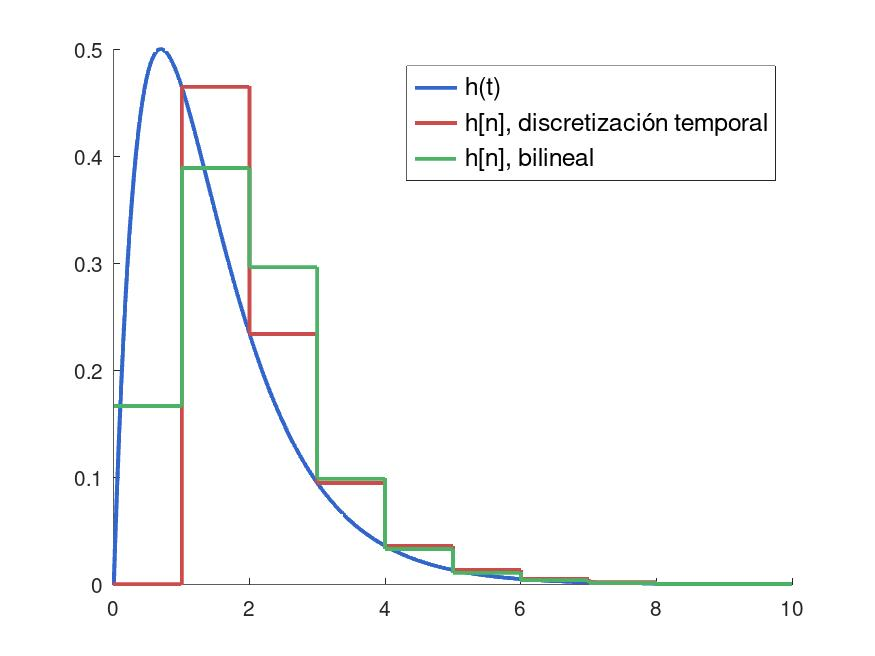
\includegraphics[width=0.7\linewidth]{./images/ej7.1.jpeg}
                \caption{Comparación de respuestas al impulso. $T = 1s$}
                \label{fig:comparacion}
              \end{figure}
              \begin{figure}[H]
                \centering
                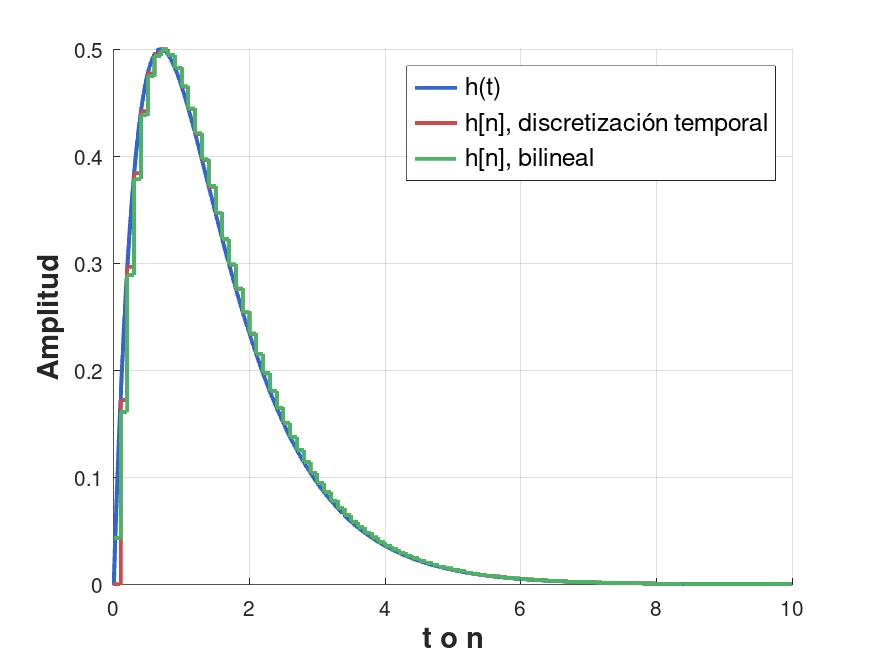
\includegraphics[width=0.7\linewidth]{./images/ej7.2.jpeg}
                \caption{Comparación de respuestas al impulso. $T = 0.1s$}
                \label{fig:comparacion}
              \end{figure}


            \item \fs{} Comparar los TVI y TVF para ambas respuestas, continua y discreta.\\
              \begin{table}[h!]
                  \centering
                  \begin{minipage}{0.45\textwidth}
                      \begin{tabular}{|c|c|c|}
                          \hline
                          \multicolumn{3}{|c|}{\textbf{TVI}} \\ \hline
                          \textbf{Continua:} & \multicolumn{2}{|c|}{$h_{(0^+)}=0$} \\ \hline
                          \textbf{Discreta:} & \textbf{Directa} & \textbf{Bilineal} \\ \hline
                          $T=1s$ & $h_{[0]}=0$ & $h_{[0]}=\frac{1}{6}$ \\ \hline
                          $T=0.1s$ & $h_{[0]}=0$ & $h_{[0]}=\frac{1}{231}$ \\ \hline
                      \end{tabular}
                  \end{minipage}
                  \hspace{5mm}
                  \begin{minipage}{0.45\textwidth}
                      \centering
                      \begin{tabular}{|c|c|c|}
                          \hline
                          \multicolumn{3}{|c|}{\textbf{TVF}} \\ \hline
                          \textbf{Continua:} & \multicolumn{2}{|c|}{$\displaystyle \lim_{n \to \infty}h_{(n)}=0$} \\ \hline
                          \textbf{Discreta:} & \textbf{Directa} & \textbf{Bilineal} \\ \hline
                          $T=1s$ & $\displaystyle \lim_{n \to \infty}h_{[n]}=0$ & $\displaystyle \lim_{n \to \infty}h_{[n]}=0$\\ \hline
                          $T=0.1s$ & $\displaystyle \lim_{n \to \infty}h_{[n]}=0$ & $\displaystyle \lim_{n \to \infty}h_{[n]}=0$ \\ \hline
                      \end{tabular}
                  \end{minipage}
                  \caption{Comparación TVI y TVF para $h$}
                  \label{tab:ejemplo}
              \end{table}

              \begin{table}[H]
                  \centering
                  \begin{minipage}{0.45\textwidth}
                      \begin{tabular}{|c|c|c|}
                          \hline
                          \multicolumn{3}{|c|}{\textbf{TVI}} \\ \hline
                          \textbf{Continua:} & \multicolumn{2}{|c|}{$y_{(0^+)}=0$} \\ \hline
                          \textbf{Discreta:} & \textbf{Directa} & \textbf{Bilineal} \\ \hline
                          $T=1s$ & $y_{[0]}=0$ & $y_{[0]}=\frac{1}{6}$ \\ \hline
                          $T=0.1s$ & $y_{[0]}=0$ & $y_{[0]}=\frac{1}{231}$ \\ \hline
                      \end{tabular}
                  \end{minipage}
                  \hspace{5mm}
                  \begin{minipage}{0.45\textwidth}
                      \centering
                      \begin{tabular}{|c|c|c|}
                          \hline
                          \multicolumn{3}{|c|}{\textbf{TVF}} \\ \hline
                          \textbf{Continua:} & \multicolumn{2}{|c|}{$\displaystyle \lim_{n \to \infty}y_{(n)}=1$} \\ \hline
                          \textbf{Discreta:} & \textbf{Directa} & \textbf{Bilineal} \\ \hline
                          $T=1s$ & $\displaystyle \lim_{n \to \infty}y_{[n]}=0.85$ & $\displaystyle \lim_{n \to \infty}y_{[n]}=1$\\ \hline
                          $T=0.1s$ & $\displaystyle \lim_{n \to \infty}y_{[n]}=9.98$ & $\displaystyle \lim_{n \to \infty}y_{[n]}=1$ \\ \hline
                      \end{tabular}
                  \end{minipage}
                  \caption{Comparación TVI y TVF de $y_{[n]}$ para $x_{[n]}={\mu_{[n]}}$}
                  \label{tab:ejemplo}
              \end{table}
            \item \fs{} Bosquejar el diagrama de BODE correspondiente para los dos filtros, y determimar $\omega_c$
                del filtro.\\
              \begin{figure}[H]
                \centering
                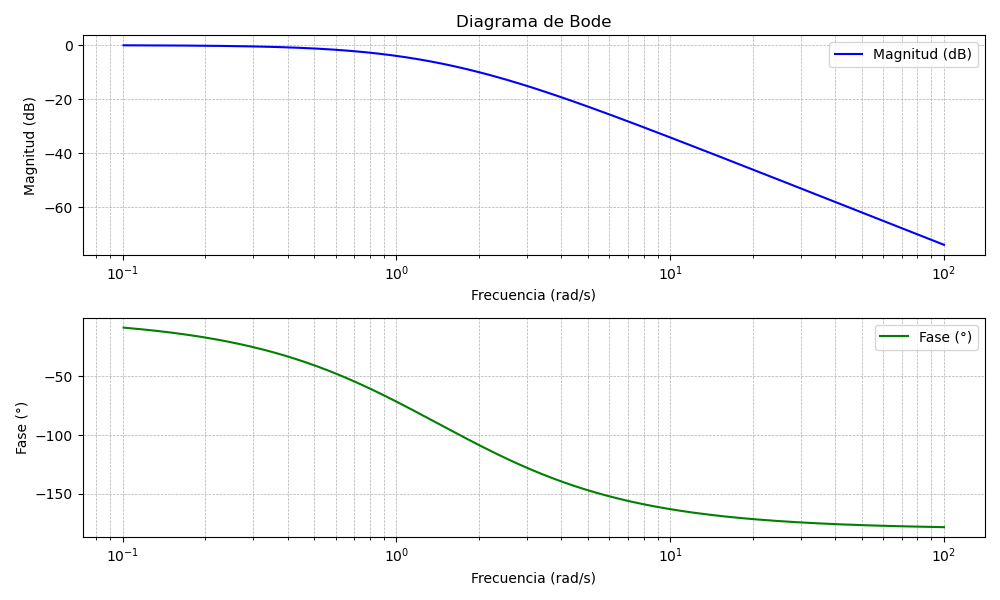
\includegraphics[width=1\linewidth]{./images/BodeHs.png}
                \caption{Diagrama de Bode para $H_s$}
              \end{figure}
              \begin{figure}[H]
                \centering
                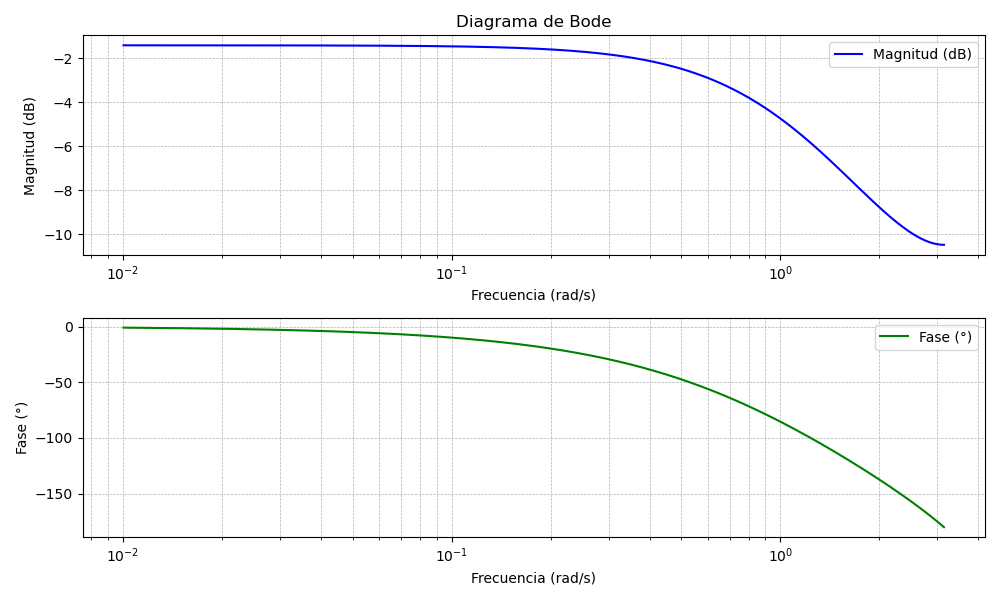
\includegraphics[width=1\linewidth]{./images/BodeD1.png}
                \caption{Diagrama de Bode para la discretizacion temporal con $T=1s$}
              \end{figure}
              \begin{figure}[H]
                \centering
                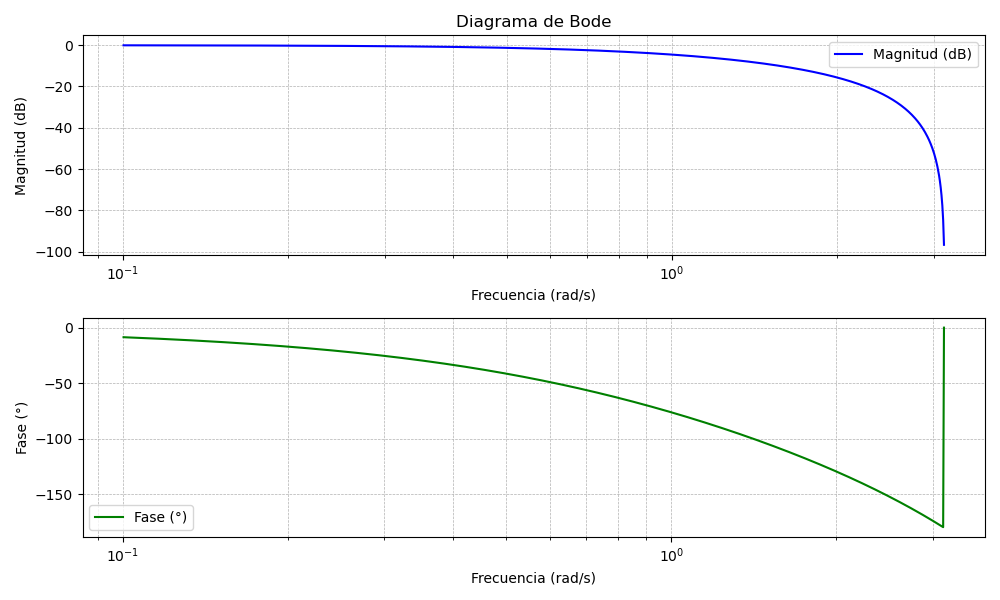
\includegraphics[width=1\linewidth]{./images/BodeB1.png}
                \caption{Diagrama de Bode para la tansformacion bilineal con $T=1s$}
              \end{figure}
              \begin{figure}[H]
                \centering
                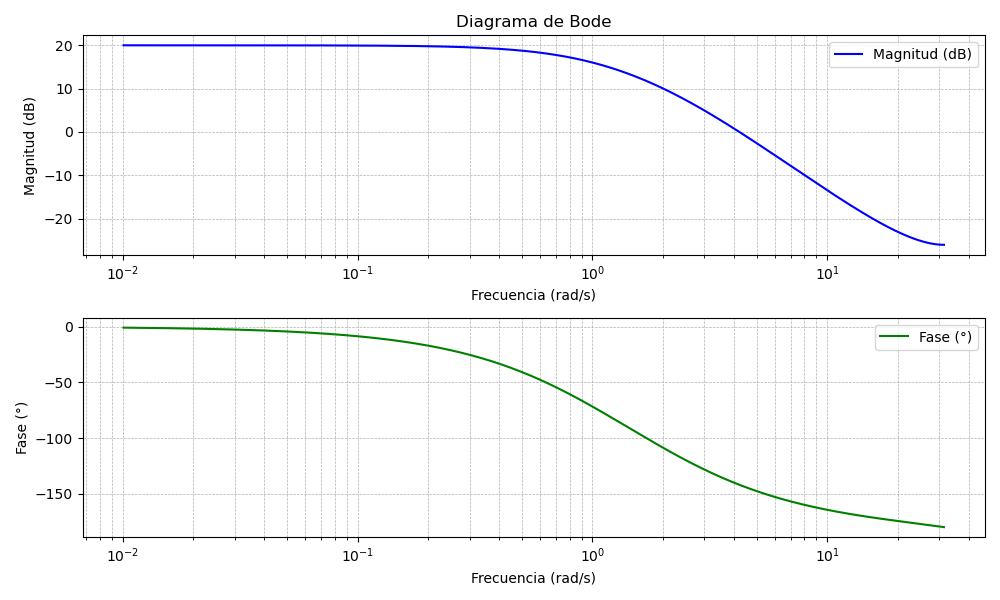
\includegraphics[width=1\linewidth]{./images/BodeD2.png}
                \caption{Diagrama de Bode para la discretizacion temporal con $T=0.1s$}
              \end{figure}
              \begin{figure}[H]
                \centering
                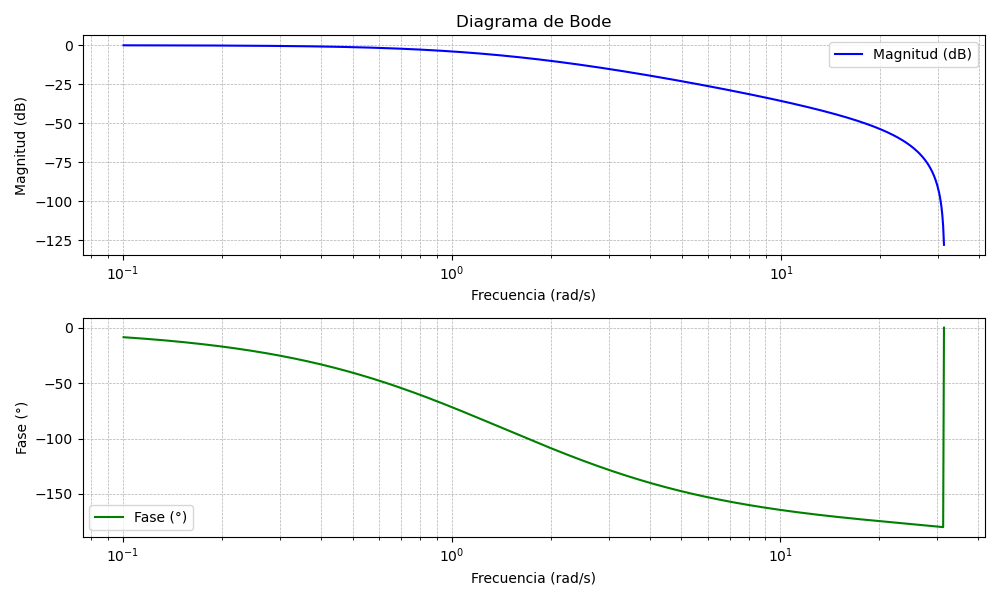
\includegraphics[width=1\linewidth]{./images/BodeB2.png}
                \caption{Diagrama de Bode para la tansformacion bilineal con $T=0.1s$}
              \end{figure}

              Para encontrar la frecuencia de corte $\omega_c$ buscamos el corte con los $-3dB$
              en el diagrama de amplitud-frecuencia para $H_s$ obteniendo:
              $$\omega_c=0.84 \hspace{1mm} rad/s$$

            \item \fs{} De acuerdo a los resultados obtenidos, ¿Que tipo de filtro es?\\

                Para determinar el tipo de filtro, consideramos la respuesta en frecuencia:
                \begin{itemize}
                    \item En bajas frecuencias (\(s \to 0\)):
                        \[
                        H(s) \approx 1,
                        \]
                        lo que indica que permite el paso de señales de baja frecuencia.

                    \item En altas frecuencias (\(s \to \infty\)):
                        \[
                        H(s) \to 0,
                        \]
                        lo que indica que atenúa las señales de alta frecuencia.
                \end{itemize}
                Esto es característico de un \textbf{filtro pasabajos}.

        \end{enumerate}

\end{document}
